

\begin{figure}
    \centering
    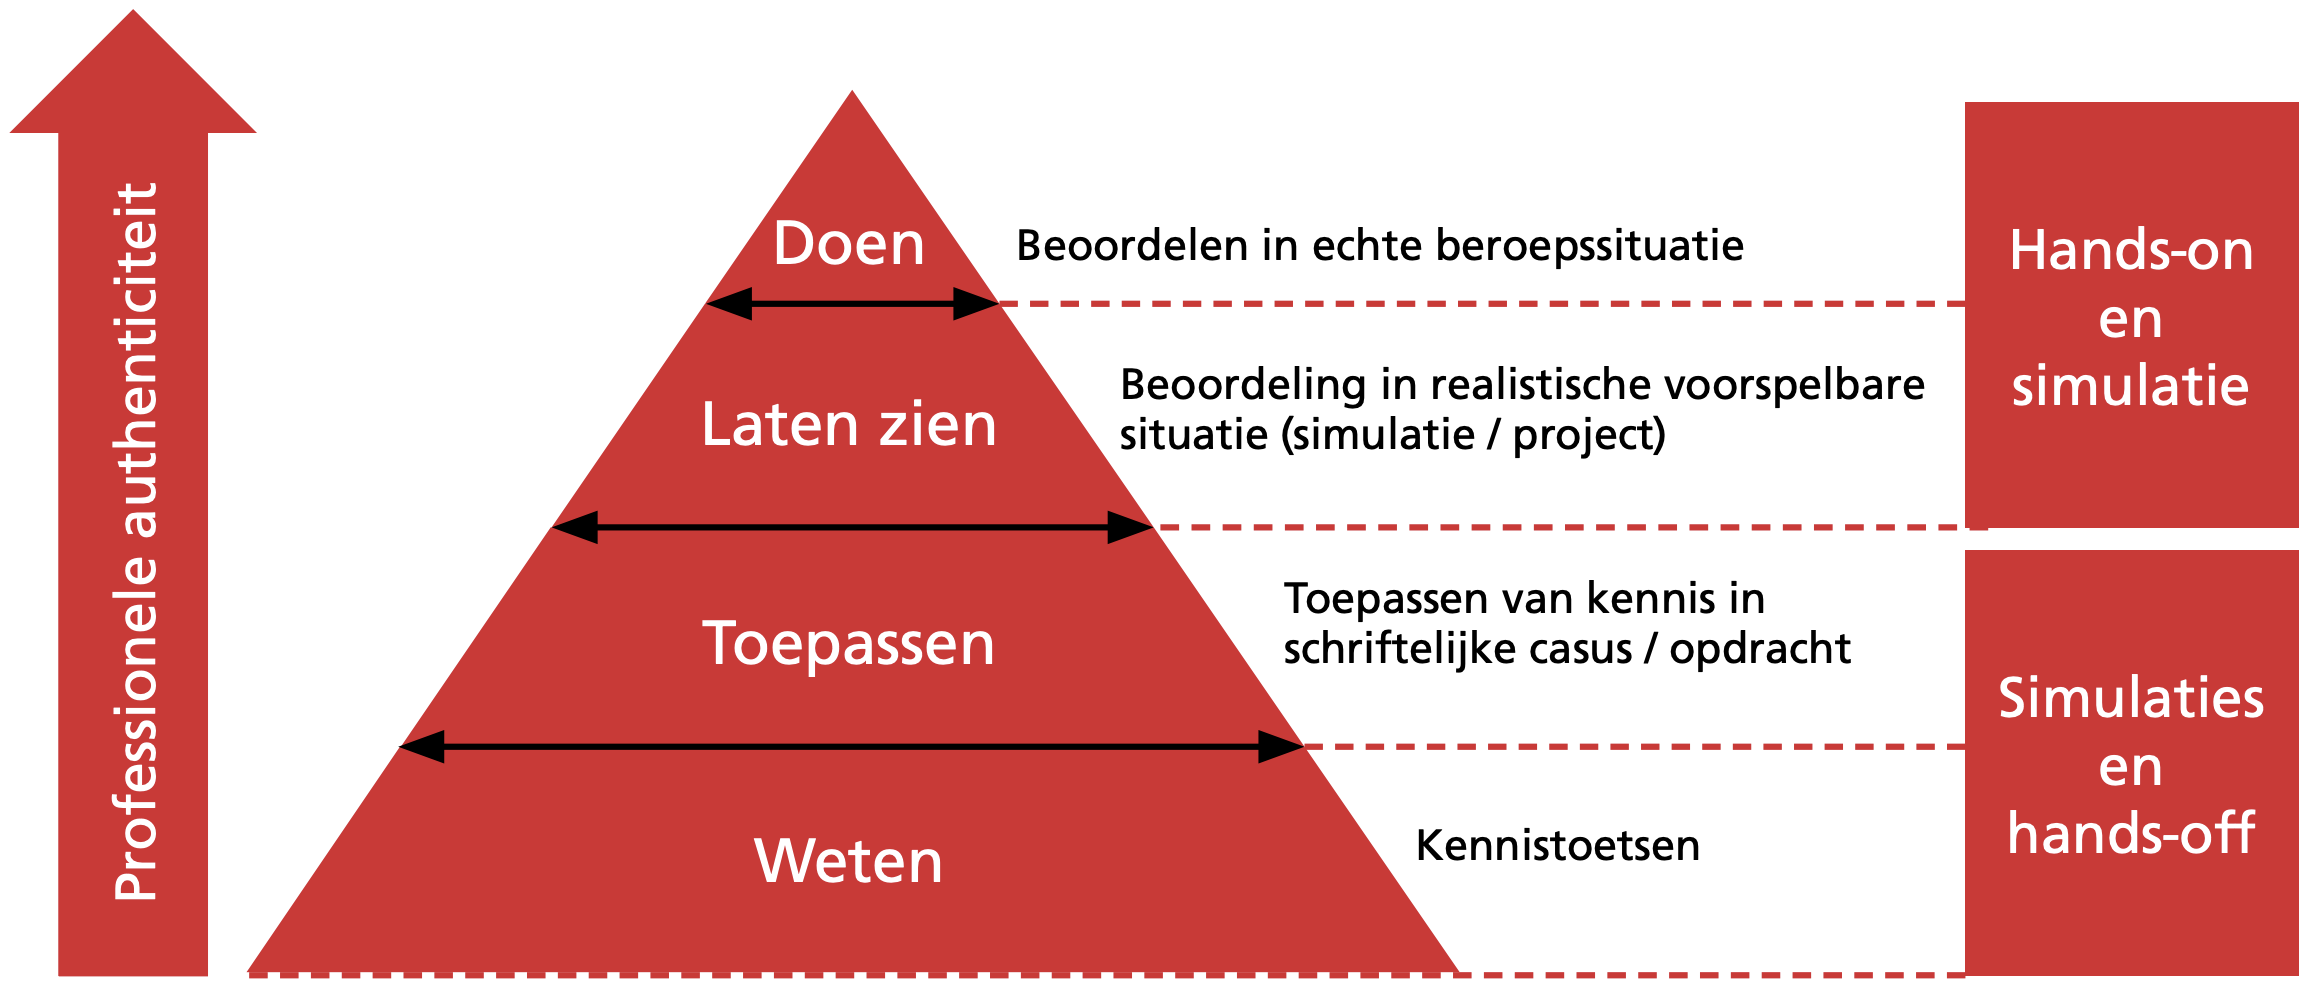
\includegraphics[width=\textwidth]{figures/miller_pyramid.png}
    \caption{Miller's pyramid~\cite{toetskwaliteit2014}}
    \label{fig:miller}
\end{figure}

While the assessment matrix and guidelines are essential to ensure a correlated assessment throughout the students, I was surprised to find out from the first iteration of the course that it was missing. 
I believe that these components do not only validate the assessment but, together with the learning outcomes, it also helps the students to gain insight into their learning process. 
Furthermore, by explicitly describing and publishing assessment criteria and bringing it to the attention of students, the assessment becomes transparent, a crucial assessment quality criteria.
\\\\
After analysing the test quality principles, a test program was developed. The Miller's pyramid which layers student progress from testing cognitive skills to practical performance was employed~\cite{toetskwaliteit2014}. 
A graphical representation of this program is shown in \cref{fig:miller}. 
At the bottom of the pyramid, the testing program implies test formats that build the knowledge base.
As the student progresses up the pyramid, the complexity and authenticity is shown through practice and performance of professional tasks.
However, the pyramid levels do not have to be sequentially followed from bottom to top. 
%This does not mean that the levels in the pyramid are sequentially from bottom to top must be finished above. Students may first "do" something and then only start to acquire the necessary knowledge. All this depends on learning style and vision learning and the complexity of the assignment.
\\\\
\Cref{appendices:assessment} contains all developed assessment documents: \textit{guidelines}, \textit{test matrix} and \textit{assessment criteria}. Apart from the specific course topic assignment, learning outcomes objectives are also considered, all accounting equally to a total of 100\%. 
Students are also assessed on their own contribution apart from the predefined assignment requirements, as a result of \gls{scaffolding}.

\subsubsection{Some examples}
After the first week, students are expected to deliver the core architecture of the application, which implies reading input from the front end and producing an output. The following work is expected:
\begin{itemize}
    \item software engineering (including inital \acrshort{uml} diagram of the proposed solution)
    \item handling of third party tooling GraphViz
    \item unit testing 
\end{itemize} 
These deliverables are re-worked thought the project and enhanced with new features. The feedback session after the fist assignment is essential in understanding studnet's competences and feedfroward for following assignments. Especially in \acrshort{ale}2 the final assignment is dependent on proper software architecture refined throughout the prior assignments to properly implement it. 